% com-cas-poster
% by hk, rj, June 2012

\documentclass[final]{beamer} 

\mode<presentation> {  
    %\usetheme{Warsaw}
    \usetheme{Boadilla}
    %\usetheme{Montpellier}
    %\usetheme{Singapore}
    %\usetheme{Ilmenau}
    %\usetheme{Berkeley}
    %\usetheme{Madrid}
}

\usepackage[english]{babel}
%hk% \usepackage[latin1]{inputenc}

\usepackage{epsfig}

\usepackage{amssymb}
%\usepackage{amsmath,amsthm, amssymb, latexsym}
\usefonttheme[onlymath]{serif}
\boldmath

\usepackage[orientation=landscape,size=a1,scale=1.4]{beamerposter}


\title[Categories and Mixins]{Categories as classes and mixin composition}

\author[Kredel \& Jolly]{Heinz Kredel\inst{1} and Raphael Jolly\inst{2}} 

\institute{IT-Center, University of Mannheim, Germany %,
%\email{kredel@rz.uni-mannheim.de,}
\and Databeans, Paris, France%,
%\email{raphael.jolly@free.fr}
}

%\date{Jun. 7th, 2012}


\begin{document}

  %hk: makes new page% \maketitle

\begin{frame}{} 
\vfill

\begin{columns}[t]

\begin{column}{.3\linewidth}
 
  \begin{block}{\large Contents}
{\normalsize 
  \begin{enumerate}
  \item generic, strongly typed, object oriented computer algebra software
  \item concept of categories 
  \item software, algorithm implementations can be packaged and
    re-combined using traits in a category-like fashion
  \end{enumerate}
\par}\par
  \end{block}
  \hfill
  \begin{block}{\large Introduction}
{\footnotesize 
The modeling of algebraic structures in a strongly typed, generic,
object oriented computer algebra software has been presented with the
systems JAS and ScAS.
The design and implementation of these strongly typed, generic and
object oriented polynomial algorithm libraries in Java and Scala is
presented in papers.  
The libraries are enhanced for interactive usage with the help of the Jython and
JRuby scripting languages. The libraries now
provide several algorithm versions for greatest common divisor,
squarefree decomposition, factorization and Gr\"obner bases
computation in separate packages.
\par}\par
  \end{block}
  \hfill
  \begin{block}{\large Related Work}
{\normalsize 
Magma [BosmaCannonPlayoust:1997] and Sage [Stein:2005], 
comments on Axiom [JenksSutor:1992,Watt:2003]\par
}\par
{\footnotesize\bf Acknowledgments}\par
{\footnotesize Thomas Becker, Wolfgang K. Seiler, Thomas Sturm, Axel Kramer, 
Jaime Gutierrez, Sherm Ostrowsky, Markus Aleksy\par}
\par
  \end{block}
  \hfill
  \begin{block}{\large Comparison with Magma and Sage}
      \centering
      {\tiny tiny}\par
      {\scriptsize scriptsize}\par
      {\footnotesize footnotesize}\par
      {\normalsize normalsize}\par
      {\large large}\par
      {\Large Large}\par
      {\LARGE LARGE}\par
  \end{block}

\end{column}

\begin{column}{.3\linewidth}
 
  \begin{block}{\large Generic, strongly typed, object oriented computer algebra software}
      \centering
      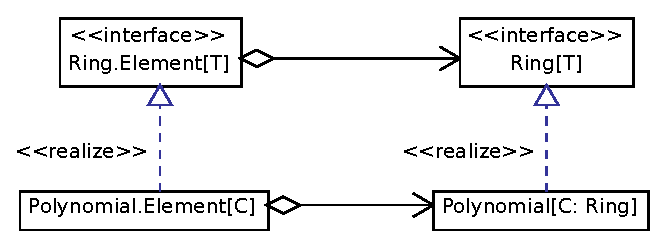
\epsfig{file=BasicTypes,clip=,width=0.55\linewidth}
\par
% want left
%{\small %/ here element = factory
%hk: does not work:
%\begin{verbatim} 
%  BigRational rf = new BigRational(1); 
%  GenPolynomialRing<BigRational> pf 
%   = new GenPolynomialRing<BigRational>(rf,new String[]{ "w" });
%  GenPolynomial<BigRational> a = pf.parse("w^2 - 2");
%\end{verbatim}
%}
  \end{block}
  \hfill
  \begin{block}{\large Algorithm libraries}
      \centering
      {\tiny tiny}\par
      {\scriptsize scriptsize}\par
      {\footnotesize footnotesize}\par
      {\normalsize normalsize}\par
      {\large large}\par
      {\Large Large}\par
      {\LARGE LARGE}\par
  \end{block}

\end{column}

\begin{column}{.3\linewidth}
 
  \begin{block}{\large Mixins for category-like software organization}
      \centering
      {\tiny tiny}\par
      {\scriptsize scriptsize}\par
      {\footnotesize footnotesize}\par
      {\normalsize normalsize}\par
      {\large large}\par
      {\Large Large}\par
      {\LARGE LARGE}\par
  \end{block}
  \hfill
  \begin{block}{\large Mixins, Traits and interfaces}
      \centering
      {\tiny tiny}\par
      {\scriptsize scriptsize}\par
      {\footnotesize footnotesize}\par
      {\normalsize normalsize}\par
      {\large large}\par
      {\Large Large}\par
      {\LARGE LARGE}\par
  \end{block}
  \hfill
  \begin{block}{\large Peer (mixin) vs hierarchical composition}
      \centering
      {\tiny tiny}\par
      {\scriptsize scriptsize}\par
      {\footnotesize footnotesize}\par
      {\normalsize normalsize}\par
      {\large large}\par
      {\Large Large}\par
      {\LARGE LARGE}\par
  \end{block}
  \hfill
  \begin{block}{\large Classes, mixin composition and categories}
      \centering
      {\tiny tiny}\par
      {\scriptsize scriptsize}\par
      {\footnotesize footnotesize}\par
      {\normalsize normalsize}\par
      {\large large}\par
      {\Large Large}\par
      {\LARGE LARGE}\par
  \end{block}

\end{column}

\end{columns}

\vfill
\end{frame}

\end{document}
